% TODO metre les noms des diapos 
\section{Resultats}
\begin{frame}
    \begin{figure}
        \centering
        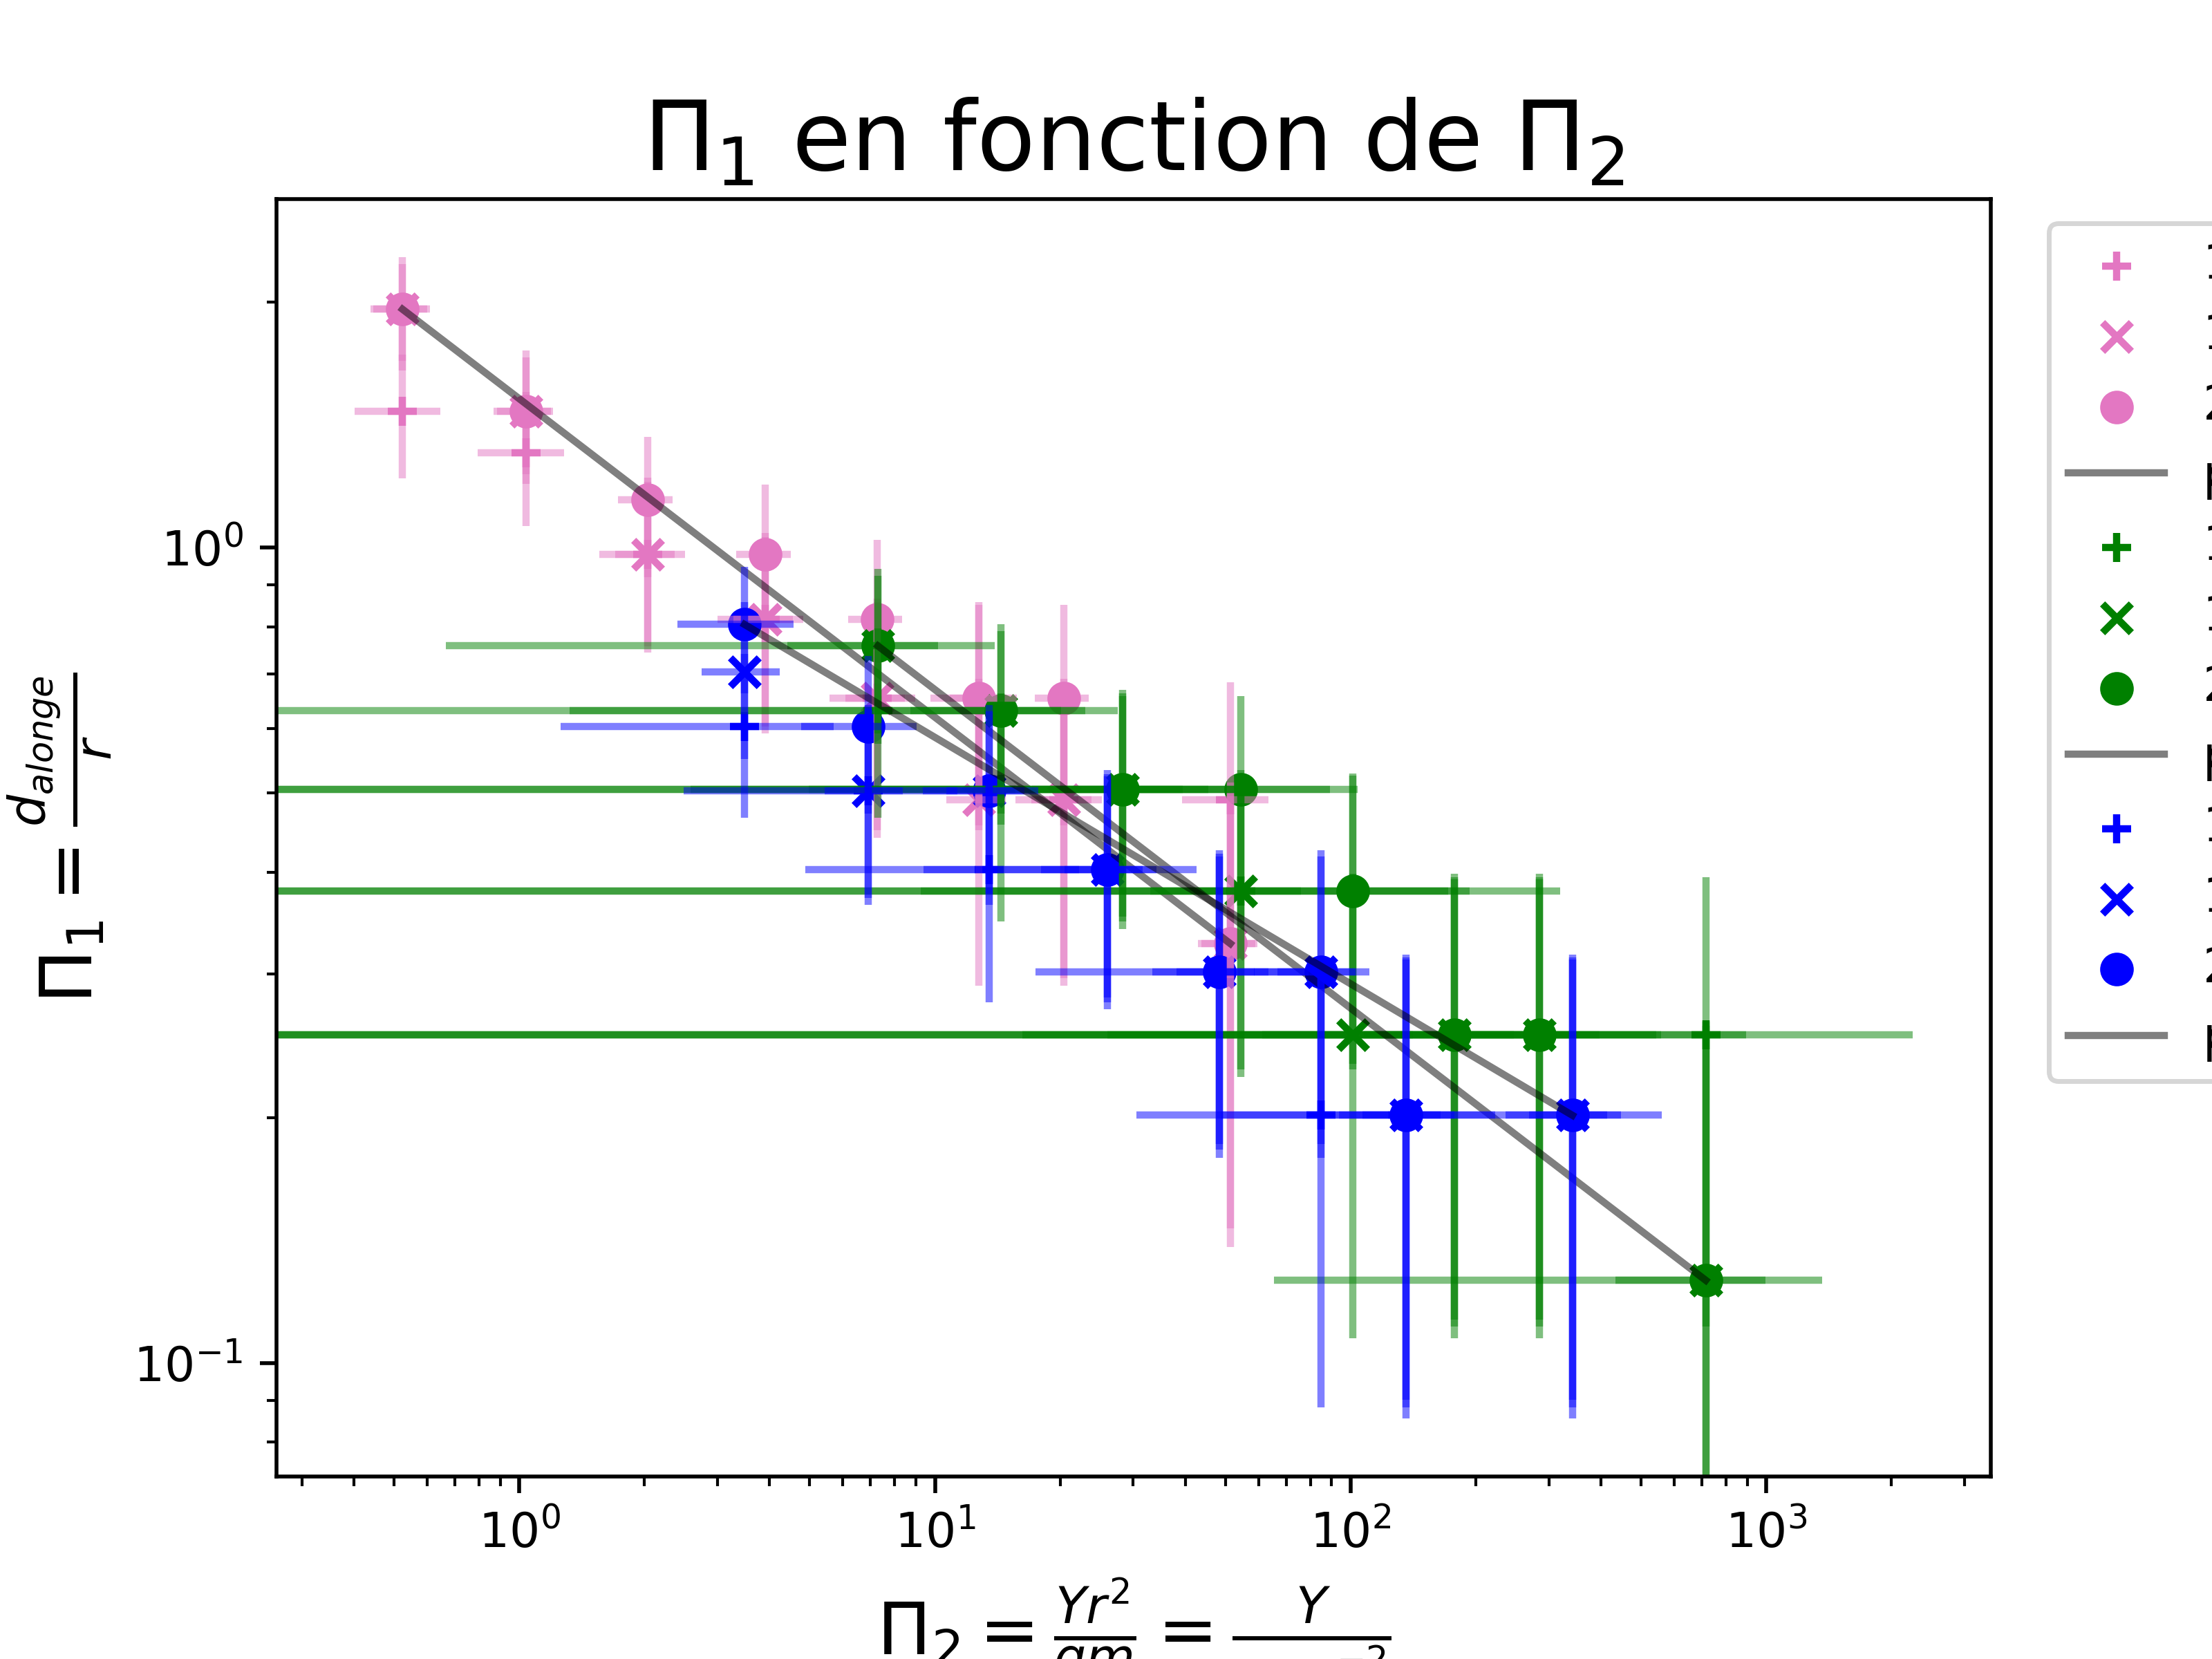
\includegraphics[height=0.9\textheight]{../Tous.png}
        \caption{A metre une caption} % TODO 
        \label{fig:my_label}
    \end{figure}
\end{frame}

\begin{frame}
    \begin{figure}
        \centering
        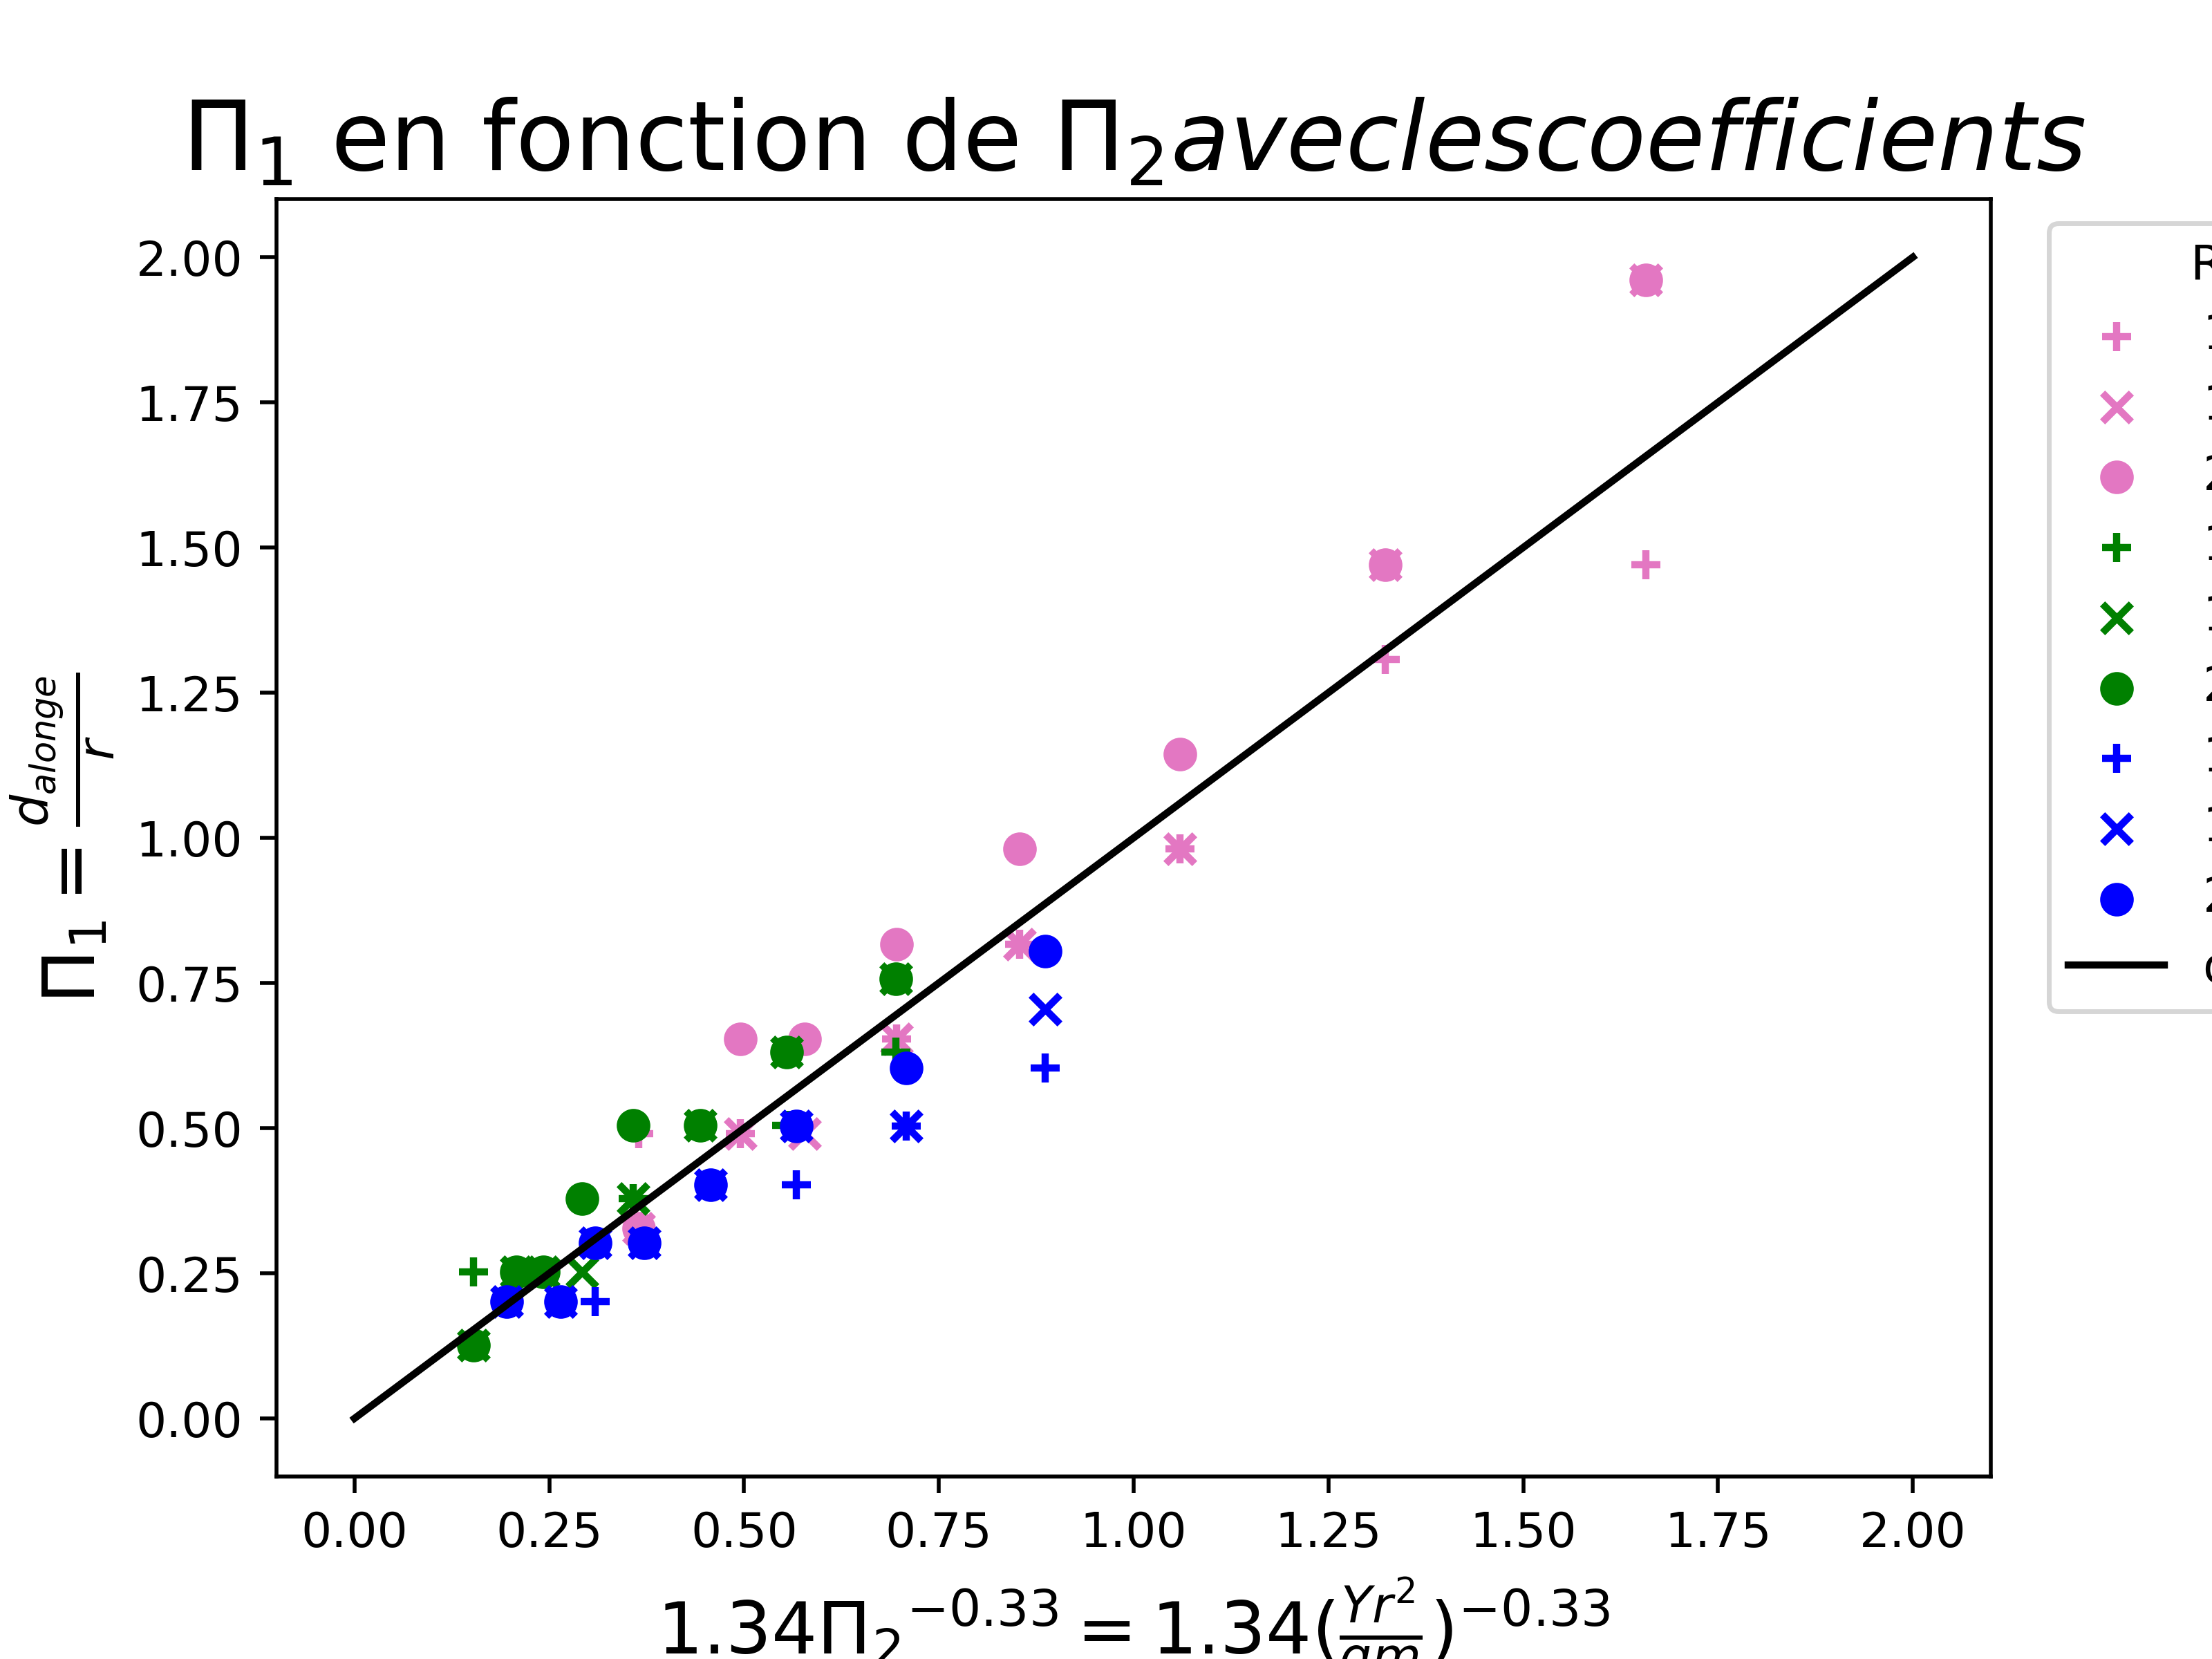
\includegraphics[height=0.9\textheight]{../Ultime.png}
        \caption{A metre une caption} % TODO 
        \label{fig:my_label}
    \end{figure}
\end{frame}

\section{La formule}
\begin{frame}{La fonction}
    \begin{block}{Fonction}
        \begin{center}
            \(d_{alongé}=1.38\cdot r\cdot\sqrt[3]{\frac{g\cdot m}{Y\cdot r^2}}=1.38\cdot \sqrt[3]{\frac{g\cdot m \cdot r}{Y}}\)
        \end{center}
    \end{block}
\end{frame}